\chapter{Toolchain Issues \label{chap:Issues}}
While the toolchain should be used in the way described in the previous chapter, there are some issues that exist in the current implementation of the toolchain that will be outlined here.
\section{LLVM Compilation}
When running the python script, a number of errors that prevent compilation do come up. First, the LLVM compilation itself can fail due to a bug in the DSWP algorithm that causes loop headers to be used as exit blocks, an example of this error can be seen in Figure \ref{fig:dswp_compile_fail}. This is likely due to missed cases when performing the partitioning of the program graph into hardware and software. The exact location of this oversight is still unknown.

\begin{figure}
	\centering
		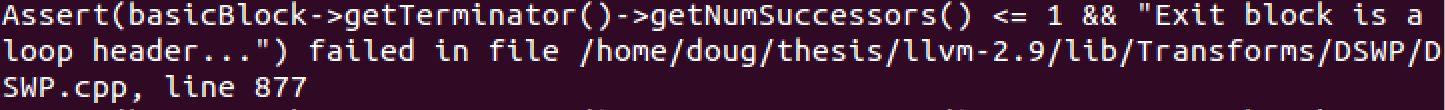
\includegraphics[width=\textwidth]{figures/DSWP_Compilation_Failure}
	\caption{Assertions Failing Within DSWP Algorithm\label{fig:dswp_compile_fail}}
\end{figure}

In order to progress past this issue in the toolchain, the amount of the program going into hardware can be configured to be a different amount, which moves where the partitioning occurs and can allow the compilation to complete successfully.